\chapter{Assessing European Preparedness for Cyber Warfare: A Comparative Analysis of France, Estonia, Germany, and the Netherlands}


\section{Introduction}
The selection of Estonia, France, Germany, and the Netherlands for our cyber defence analysis is rooted in their pivotal roles within the European Union's strategic framework, despite embracing diverse approaches to cybersecurity. This strategic diversity spans from Estonia, recognized for its extensive experience as a cyber defender, to the Netherlands, France, and Germany, major players in European Union politics. The inclusion of these nations in our study is driven by their influential positions and distinct cybersecurity strategies, offering a comprehensive spectrum of perspectives within the European landscape.

These countries not only showcase varied cyber defence tactics but also hold strategic significance in the European Union's overarching cybersecurity initiatives. Their diverse approaches, ranging from proactive cyber defence measures to nuanced political engagements, contribute to a comprehensive understanding of cybersecurity challenges and strategies at both regional and international levels. Furthermore, the selection is informed by the wealth of official documents and publicly accessible data available from these nations. 

\begin{figure}[H]
    \centering
    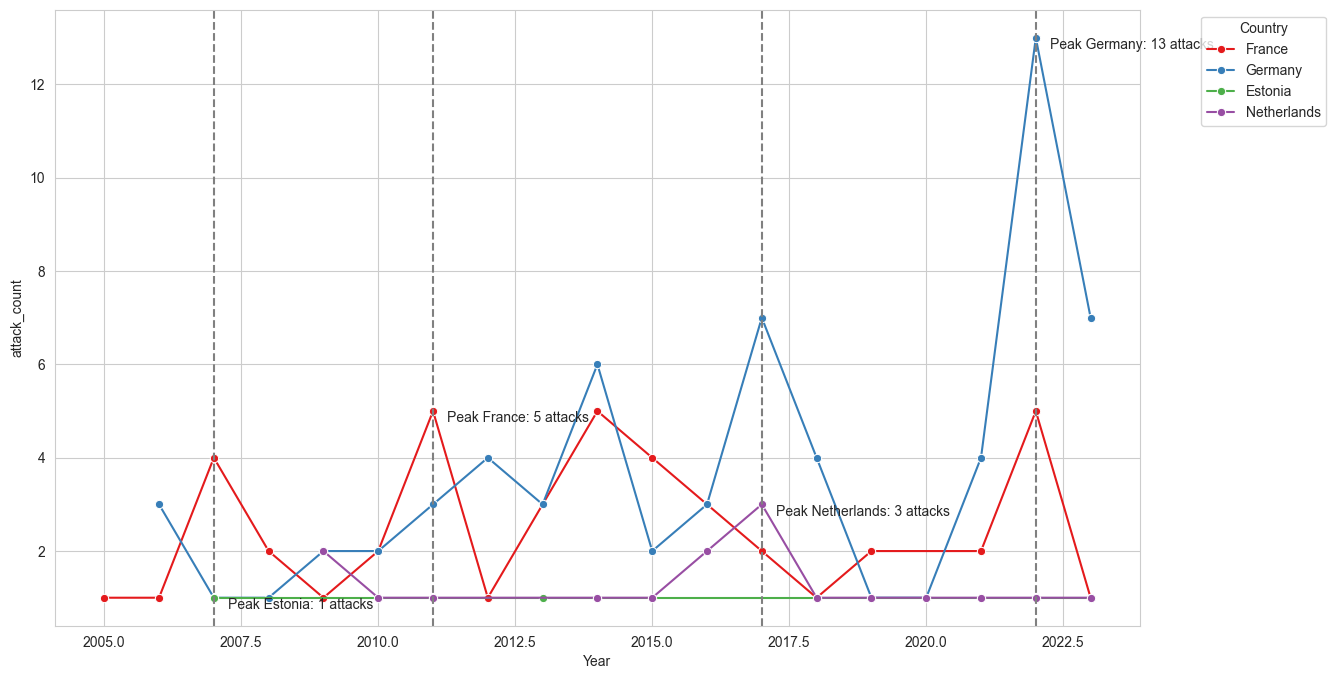
\includegraphics[width=1\textwidth]{Images/attack_countries.png}
    \caption{\textit{Number of State-sponsored cyber operations 2005-2023}}
        \source{Source: \autocite{eurepoc2023}}
    \label{fig:attack_countries}
\end{figure}

The line plot in Figure \ref{fig:attack_countries} depicts the landscape of state-sponsored cyberattacks experienced by the analysed countries. The data was obtained through exploratory data analysis from the EuRepoC dataset, and a table with years and cyberattacks is provided in Appendix \ref{tab:cyberattacks_per_year}.

Germany has encountered more cyber operations than its counterparts, experiencing a significant surge after the war in Ukraine. Germany is considered the most active European country in providing military support to Ukraine, and it holds a crucial position as a political and economic player, not only within the European context but also on the global stage. Furthermore, France follows Germany closely in terms of the number of attacks. The increased frequency of attacks is not directly linked to an inability to counter them but rather to the overall number of attacks, given that attack vectors can have a multiplied effect in a larger and more connected economy.

Estonia and the Netherlands, on the other hand, have faced fewer attacks. Specifically, Estonia has drawn valuable lessons from the 2007 attacks, contributing to an enhancement of its preparedness. Additionally, the smaller size of its economy and state support contribute to a more defensive approach.

Russia has been the most attributed country for cyberattacks in Estonia and Germany, while China is associated with attacks in France and the Netherlands \ref{cod:attacker}.

\begin{figure}[H]
    \centering
        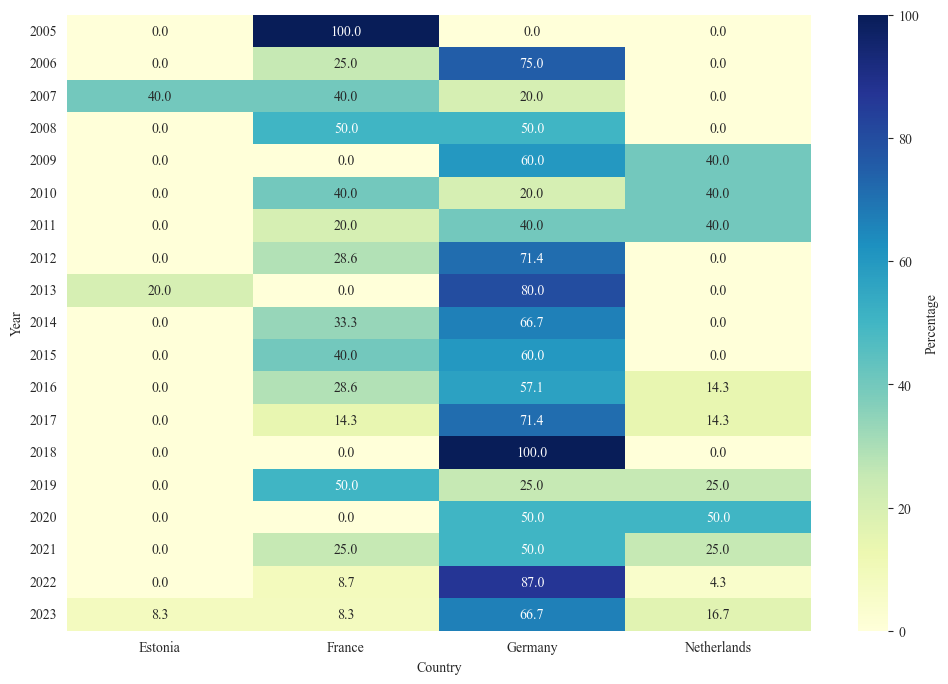
\includegraphics[width=1\textwidth]{Images/disruption.png}
        \caption{\textit{Percentage of disruption after State-sponsored cyber operations 2005-2023}}
        \source{Source: \autocite{eurepoc2023}}
        \label{fig:disruption}
\end{figure}


Furthermore, another analysis has been conducted regarding the disruption caused by the attacks. Mostly, the countries have experienced an improvement over the years, as associated with low disruption in cyberattacks, as depicted in Figure \ref{fig:disruption}. However, it is important to note that Germany has not only encountered a higher number of cyberattacks but also more disruption resulting from them. This highlights the probability of Germany being a crucial target for foreign cyber operations while possessing fewer capabilities to counter them.

Following this overview, the chapter will delve specifically into the cyberstrategies of the analyzed countries, aiming to gain insights into how these nations are influencing changes in cyber strategies after the war in Ukraine and what challenges lie ahead.


\section{France}

This section offers a comprehensive exploration of France's cyber defence strategy, meticulously outlined in the Strategic Review of Cyber Defence \autocite{sgdsn_2018_strategic}. By dissecting key components such as operational chains, governance structures, and specific doctrines, we aim to uncover the interconnected layers that constitute France's resilient stance against evolving cyber threats.

In February 2018, France released a White Paper, signalling a strategic shift in its approach to cyber defence. Beyond a mere enumeration of operational chains and governance bodies, this analysis seeks to unravel the cohesive strategy that guides France's response to the dynamic cyber threat landscape.

France's cyber defence strategy unfolds through four operational chains, each with a distinct role. The Protection Chain, spearheaded by SGDSN and ANSSI, stands as the frontline defence for national security during cyberattacks. Complementing this, the Military Action Chain provides the President with the authority to deploy cyber warfare in the interest of national defence. Simultaneously, the intelligence chain focusses on attribution of cyberattacks, while the judiciary investigation chains involve law enforcement in the aftermath of cyber-related crimes \autocite{sgdsn_2018_strategic, anssi_2022_le}.

\begin{figure}[H]
    \centering
    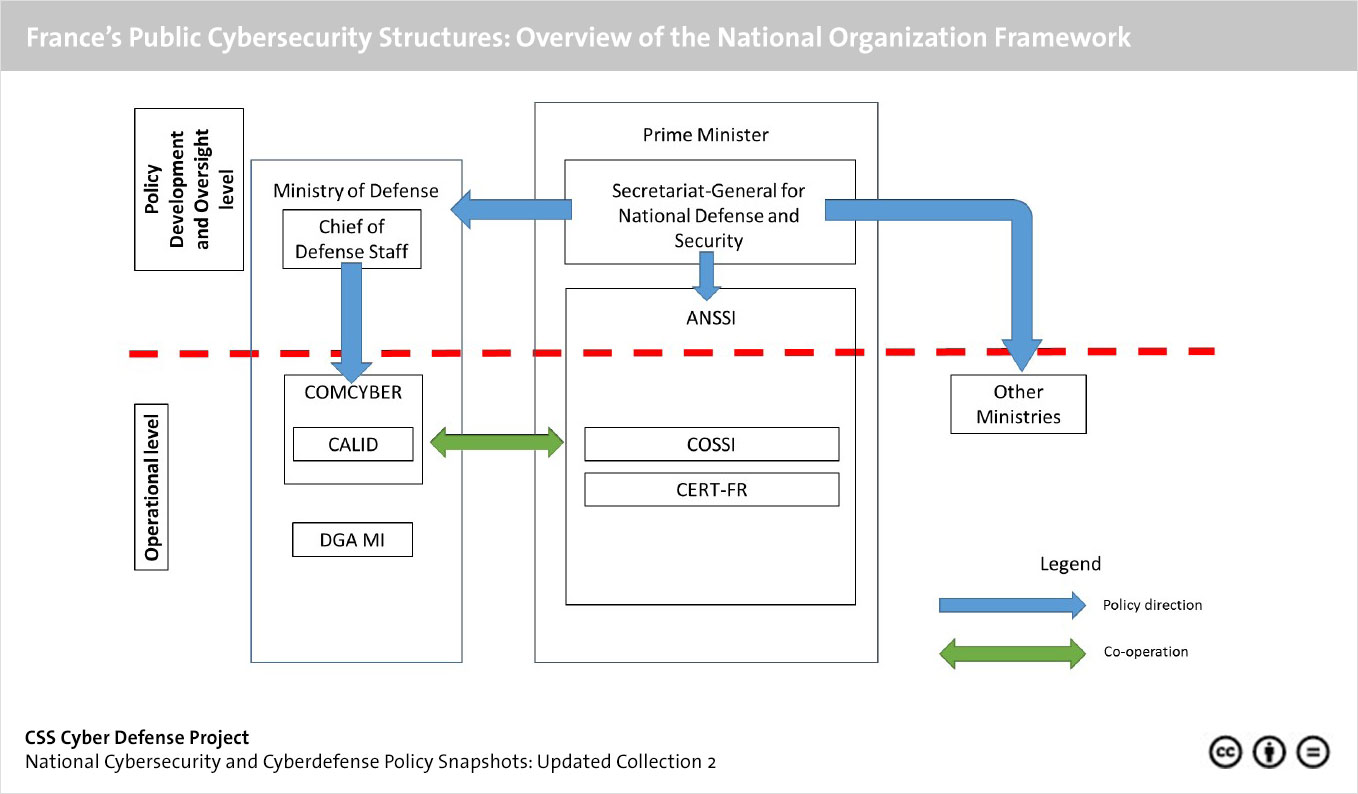
\includegraphics[width=1\textwidth]{Images/france.jpg}
    \caption{\textit{France Cyber Structure}}
        \source{Source: \autocite{sdewar_2018_national}}
    \label{fig:france}
\end{figure}

\textbf{Governance and Crisis Management}: Beyond the operational facets, France has meticulously crafted a governance structure to manage cyber crises. The Cyber Defence Management Committee, the Cyber Defence Steering Committee, and the Cyber Crisis Coordination Centre collectively orchestrate a coordinated response.  Permanent Cyber Posture (PPC) ensures uninterrupted 24/7 defence, reflecting a commitment to proactive cyber defence. This interplay of structures and strategies exemplifies a holistic approach to cyber resilience.

\textbf{Defensive Cyber Warfare Policy (LID)}: The Defensive Cyber Warfare Policy (LID) serves as the linchpin of France's defensive capabilities. Beyond a mere list of missions, LID embodies a strategy of awareness, probability assessment, protection enhancement, detection, reaction, and attribution. The interdependence between these missions showcases a holistic approach to safeguarding national interests. Moreover, the emphasis on collaboration, exemplified by the Network and Information Systems Directive (NIS) and its updated version (NIS2), emphasizes the importance of unified efforts between electronic communication operators, web hosts, and national entities. Local level involvement through coordination forums further cements the idea of a collective defence \autocite{ministredesarmes_2019_politique}.

\textbf{Offensive Cyber Warfare Doctrine (LIO)}: In tandem with defensive measures, France has integrated offensive capabilities within its overall military strategy through the Offensive Cyber Warfare Doctrine (LIO). COMCYBER, operating under the Chief of Staff of the Armed Forces, oversees the orchestration of LIO. By acknowledging the necessity for political, legal, and military risk evaluations, France strikes a delicate balance between secrecy and transparency. The democratic nature of the state guides decisions on the disclosure of LIO actions \autocite{ministredesarmes_2019_lments}.

\textbf{Influence Computer Control (L2I)}: Expanding beyond national borders, France recognizes the importance of information warfare through the Influence Computer Control (L2I). Executed by CYBERCOM, L2I operations aim to detect and counter information attacks, gather intelligence, and engage in deception operations. Challenges, such as the investment in human resources, are met head-on through the Military Program Law 2019-2025, allocating resources for cyber fighters and acknowledging the financial commitment needed \autocite{ministredesarmes_2021_lments}.

France identifies private companies or public bodies that are of vital importance. The \textit{Secteur d'activité d'importance vital} applies to these, a provision which raises the level of security in the event of an attack, including cyberattacks. Due to the increase in cyberattacks, the provision has been transformed specifically for vital information systems (making information systems a separate category of cyber infrastructure). To date, more than 200 entities have been labelled as such with the obligation to notify any incident, as well as apply more stringent crisis prevention and management measures \autocite{anssi_2022_le}.

In conclusion, France's cyber defence strategy is a tapestry woven with interconnected threads, each playing a crucial role in ensuring national cybersecurity. By delving beyond the surface enumeration of strategies, this analysis unravels the symbiotic relationship between operational chains, governance structures, and specific doctrines. In an era of evolving cyber threats, France's adaptive and integrated approach stands as a model for nations navigating the complex landscape of digital security. Furthermore, France has increased its awareness and cyber capabilities even before the War in Ukraine, anticipating strategies on the involvement of public sector in the cyber defence and the use of offensive attacks in their doctrine. However, no public available information for the integration of cyber and kinetic weapons were found. 

\section{Estonia}
Estonia experiences with cyberattacks has shaped not only its own strategy but also became a successful model of how to exploit security vulnerabilities to improve its readiness to counter future attacks. After 2007, Estonia have developed a multifaced cyber strategy, an outcome from a continuous learning and development of proactive defence measures. 

\textbf{National Security concerns} Unlike the other countries analysed in this dissertation, Estonia is more familiar with a real threat that combines kinetic and cyber operations from non-state actors (supported from Russia). In this regard, the National Security Concept published in 2017 highlight that Estonia applies measures to guarantee the digital continuity of the state even in situations where it has lost the control over its territory \autocite[16]{republicofestonia_2017_national}. For a small state like Estonia, the synergy between the private sector, the civil society and the State becomes a priority.  

As well as in the previous analysis, the main challenge that Estonia must tackle regards the skill and specialization. Even the flexibility of being a small country helps professionals to connect with each other and create communities which are valuable in the cyber domain, this approach to the crisis management could not be sustainable due to increase complex of technology risks.  

\textbf{International Cooperation \& exercises} Estonia is actively involved in the international cooperation in the cyber domain. It hosts the Cooperative Cyber Defence Centre of Excellence (CCDCOE), a NATO-accredited centre for cybersecurity and cyber defence. In fact, Tallinn CCDCOE hosts the most important NATO cyber exercises, such as the Cyber Coalition and Locked Shields. The alignment with allied military presence, particularly NATO's Enhanced Forward Presence (eFP), underscores the need for evolving cooperation mechanisms and procedures to collectively address cyber threats. Estonia aims to establish a comprehensive approach, encompassing political, legal, and technical dimensions, to attribute cyber-attacks, participate in deterrence efforts, and collaborate with like-minded countries in cyber defence frameworks \autocite{ministryofeconomicaffairsandcommunication_2019_cybersecurity}. 

The small Baltic country has also bilateral cyber exercise such as Baltic Blitz 23 with United Stated, as well as joint defensive operations with the USCYBERCOM\footnote{ Information about this operation were published by the US Cyber Command on their website: https://www.cybercom.mil/Media/News/Article/2433245/hunt-forward-estonia-estonia-us-strengthen-partnership-in-cyber-domain-with-joi/}. While Estonia official document do not mention the cyber offensive capabilities of their military, the Baltic State has been a central player in hosting NATO Crossed Swords, a redteamming exercise with the aim to explore the kinetic-cyber synergies in a wartime scenario \footnote{ Even if exercises like that are under exceptional secrecy, local media offers useful insights: https://news.err.ee/1608427058/offensive-cyber-operations-exercise-kicks-off-in-estonia}. 

\begin{figure}[H]
    \centering
    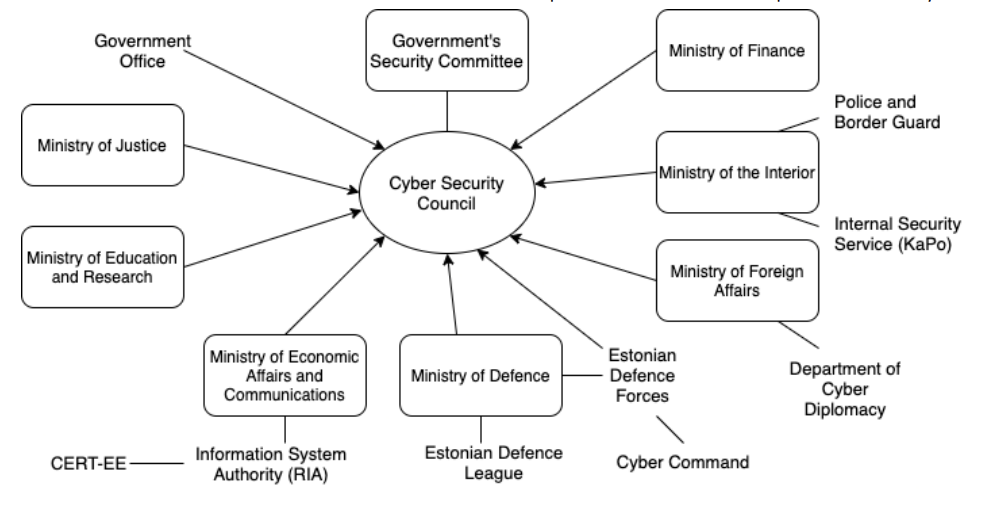
\includegraphics[width=1\textwidth]{Images/estonia.png}
    \caption{\textit{Estonia Cyber Structure}}
        \source{Source: \autocite{kohler_2020_cyberdefense}}
    \label{fig:estonia}
\end{figure}

\textbf{Cyber Military structure} From the military perspective, the Cyber Command, which become operation in 2018, have the task to carry out cyber operations and to provide cyber defence. The Cyber Command subdivisions include \autocite{defenceforces_2023_cyber}: 
\begin{itemize}
    \item ICT centre: develop the defence architecture of military forces, as well as coordinating the development in the technology domain. 
    \item Cyber Information Operation Centre: prepare the reserve units and active planning of cyber operations and defence.
\end{itemize}

Estonia represents a unique case in which a civil cyber army is officially recognized as part of the Estonian Armed Forces. The country's cyber civil defence force, which is integrated into the Estonian Defence League, is dedicated to enhancing national cyber resilience. Members of this unit typically comprise IT professionals, programmers, and individuals possessing expertise in cybersecurity. The cooperation between civil society and the state is palpable in this framework. By involving IT experts and cybersecurity specialists from outside traditional military establishments, Estonia fortifies the bond between the government and the public, thereby cultivating a shared responsibility for national cybersecurity.

Estonia embrace deterrence by denial in the cyberspace \autocite{oh_2019_exploring}. The aim is to make it difficult for attackers to achieve their objectives, thereby dissuading them from attempting cyberattacks in the first place. 

\textbf{Protection of Critical Infrastructure} For what regards the protection of critical information infrastructure, the Information System Authority (RIA) is the competent authority which encompass the cyber crisis management. Additionally, RIA works with state authorities and businesses that provide essential services to coordinate efforts to avoid and handle cyber emergencies. It also collaborates on civilian-military cyber initiatives with the Defence Forces and Defence League. Moreover, RIA coordinates the national response to significant cyber incidents, which are defined as incidents that jeopardize or negatively impact system security, in compliance with the Emergency Act. Through incident prevention, preparedness planning, and incident response coordination, RIA maintains a state of readiness by utilizing strategies like legislative advancements, security officer network management, and other training efforts. In order to prepare for large-scale cyber incidents, RIA's Incident Response Department regularly conducts risk analyses to evaluate the likelihood and consequences of such events. Depending on the type and extent of the emergency, this preparation may involve working with other cybersecurity departments and pertinent authorities listed in the Emergency Response Plan, such as the Cyber Unit of the Estonian Defence League \autocite{informationsystemauthority_2022_cyber}

Estonia plays an important role in the cyber diplomacy. The 2007 Russian cyberattacks served as a turning point, prompting Estonia to intensify its efforts in cyber diplomacy. In 2018, it appointed its first ambassador-at-large for cybersecurity, and the following year, a dedicated department was established to lead the country's cyber diplomacy initiatives \autocite{theinternationalinstituteforstrategicstudies_2023_cyber}.  



In summary, Estonia's response to cyber threats stands as a resilient model shaped by its experiences, particularly the impactful cyberattacks in 2007. This multifaceted strategy reflects a continuous commitment to learning and proactive defence. Unlike its counterparts, Estonia faces a tangible threat, blending kinetic and cyber operations from non-state actors, necessitating measures to ensure digital continuity even in the absence of territorial control.

\section{Germany}

Germany plays a central role in both economic and political spheres within the European Union. While its defence and civil industry are robust, the cybersecurity and cyberdefence sectors are still undergoing continuous development. This evolution is taking place under a centralized structure, with key responsibilities allocated to the Ministry of Interior and the Ministry of Defence. The War in Ukraine caused a sharp strategic position on boosting its military capabilities, with €100 billion, 21 of which dedicated to the improvement of communication and cyber capabilities. 

\begin{figure}[H]
    \centering
    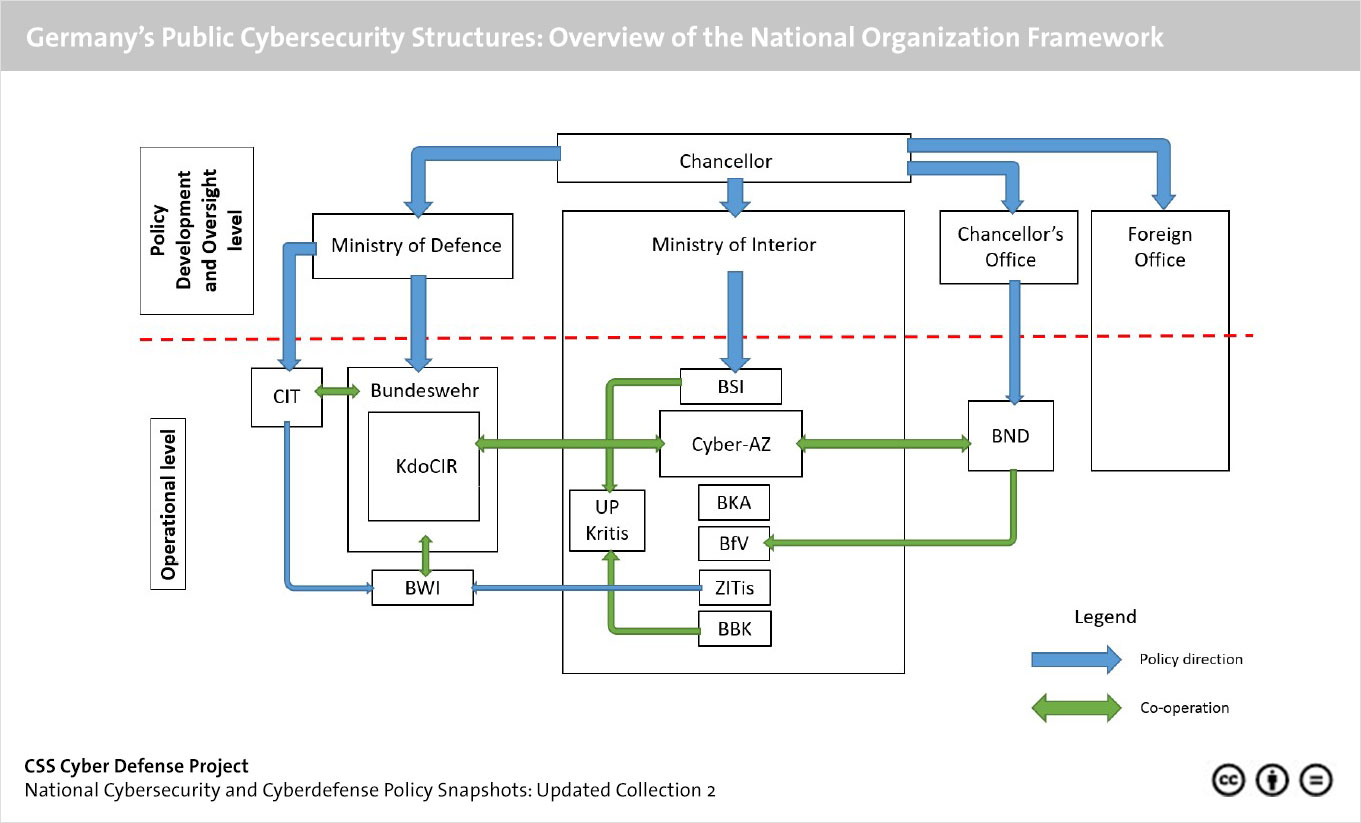
\includegraphics[width=1\textwidth]{Images/germany.jpg}
    \caption{\textit{Germany Cyber Structure}}
        \source{Source: \autocite{sdewar_2018_national}}
    \label{fig:germany}
\end{figure}

\textbf{Germany Cyber Structure} Germany's cyber-security architecture is complex, with its governance distributed between different government entities. The Federal Ministry of the Interior (BMI) controls the police forces and domestic intelligence service. Furthermore, within the Central Office for Information Technology in the Security Sector centralise the government governance role regarding cyber activities, while coordinating with the National Cyber Security Strategy (NCSS). On the other hand, the Federal Office for Information Security (BSI) sets best practices, guidelines and standards for the cybersecurity measures. \autocite{theinternationalinstituteforstrategicstudies_2023_cyber, federalministryoftheinteriorbuildingandcommunity_2021_cyber}

At the national level, the National Cyber Security Council coordinates the federal government's cyber-security policy and fosters collaboration between the public and private sectors. The Ministry of Defence (BMVg) is responsible for protecting its systems and engaging in cyber-security, including offensive cyber operations. The CIT focuses on acquiring, using, and protecting the IT infrastructure of the BMVg, the nationalized company BWI, and the Bundeswehr. Its role is to streamline responsibilities, promote technological development, and harmonize soft- and hardware capabilities. In addition, the KdoCIR operates independently of traditional military branches and is tasked with protecting critical infrastructure, conducting computer network operations, recognizing propaganda and disinformation, participating in opinion-making, and compiling military and cyber intelligence. The KdoCIR comprises two main pillars: the Strategic Reconnaissance Command (KdoStratAufkl) and IT Command of the Bundeswehr (KdoITBw). The former focuses on intelligence information management and reconnaissance in cyberspace, while the latter is responsible for IT-system operations, cybersecurity, and IT evaluation. Germany represents a forward position toward a structured cyber defense within the military domain and considered the best computer forensic expert from the NATO members \autocite{leinhos_2020_cyber}. 

The Federal Intelligence Service (BND) is Germany's primary foreign intelligence agency, engaging in cyber-intelligence operations with a focus on signals intelligence. The BND operates under a unique legal regime, conducting cyber espionage and intercepting communications. The Federal Office for the Protection of the Constitution (BfV) handles domestic intelligence, including some cyber-security and cyber-espionage functions. The Military Counter-Intelligence Service defends against attacks on the German armed forces. \autocite{theinternationalinstituteforstrategicstudies_2023_cyber, federalministryoftheinteriorbuildingandcommunity_2021_cyber}

Germany has set up a Federal Agency for Innovation in Cybersecurity, denominated \textit{Cyberagentur}, with the aim to speed up the innovation in this sector. Their strategy focuses on the development of AI systems for cybersecurity as well as applications of cryptography and quantum computing \footnote{For more information, please consult the following document: https://www.cyberagentur.de/wp-content/uploads/2023/11/Strategie-2022-2025-Internet.pdf}. 

\textbf{Offensive or Defensive capabilities?} Germany is positioned towards an active cyber defence role \autocite{federalministryoftheinteriorbuildingandcommunity_2021_cyber}. However, the German Basic Law constrains the intervention from the Bundeswehr in response to cyberattacks or their attribution, which is considered a responsibility of law enforcement agencies and intelligence services \autocite{leinhos_2020_cyber}. The defence position is focused on protecting state secret and Bundeswehr from cyber espionage and sabotage \autocite{federalministryoftheinteriorbuildingandcommunity_2021_cyber, thefederalgovernmentofgermany_2023_robust}. However, clear strategy on cyber defence from the military perspective, as well as the cyber \& kinetic integration. A critical position for strategic country such as Germany to not be ready (at least from regulatory and public strategic perspective) to have an offensive and defensive cyberstrategy applied to military domain. 

Germany opposes to the offensive cyber capabilities (the so called \textit{hackback} or preventive attack). Its position is less exposed to uncontrolled effect of offensive actions, and it is directly linked with the attribution issues that constitutes an obstacle in the definition of offensive cyber operations towards State actors \footnote{Public announcement have confirmed this position: https://www.euractiv.com/section/cybersecurity/news/german-national-security-strategy-leaves-out-cyber-counter-attacks/}.

\textbf{Protection of Critical Infrastructure} The National Cyber Response Centre have set reconnaissance and early warnings capabilities to promote situational awareness while involving stakeholders to contribute to them (national security strategy). Critical infrastructure and information ones are regulated through the \textit{National Strategy for the Protection of Critical Infrastructures} \autocite{federalofficeforinformationsecurity_2022_up} and \textit{National Plan for the Protection of Information Infrastructure}s (NPSI) respectively. The Cybersecurity strategy stress out the need to replace reactive measure with proactive ones. A problem that emerges on this page is linked to the voluntary nature of strategic entities in participating in the exchange of information, which can be fundamental for preparing for cyberattacks. On the other side, concerns appear about the European inability to guarantee competition at an institutional information level (see 5G and the smartphone market) with Asia and the US, which have built an oligopoly. This negatively affects the ability to guarantee the security of information networks not only in Germany but also in Europe. The German government is pursuing an enhanced cybersecurity framework by fostering collaboration between public sector, research community, private companies and civil society. This collaboration is, and it will be possible through projects like UP KRITIS and the National Pact on Cybersecurity. The outcomes expected are just not related to improving cyber measures but also facilitate information and skills exchange between the vertical and horizontal levels \autocite{federalofficeforinformationsecurity_2022_up, federalministryoftheinteriorbuildingandcommunity_2021_cyber, thefederalgovernmentofgermany_2023_robust}.

\textbf{Intelligence} Germany has stressed out that the settlement of preventive measures it would be possible only through intelligence gathering. This task is delegated to the Federal Office of Military Counter-intelligence (BAMAD), created to acquire information about cyber threats, understating motives, capabilities and attack vectors to prepare the victims. The work of the new counter-intelligence subdivision goes along with the cooperation with other federal intelligence agencies and the private sector \autocite{theinternationalinstituteforstrategicstudies_2023_cyber}. 

\textbf{Challenges ahead} As the other countries, Germany faces a critical challenge in recruiting talents in the cybersecurity domain \autocite{thefederalgovernmentofgermany_2023_robust, leinhos_2020_cyber}. In this regard, the cyber cluster at the \textit{Universität der Bundeswehr München} in Munich not only carries out research but also provides basic, advanced and further training for officers and Federal Government employees, with a focus on cybersecurity \autocite[25]{federalministryoftheinteriorbuildingandcommunity_2021_cyber}. Another issue regards the IT procurement and innovation of both terminals and infrastructure. Some step-forwards have been made with the modernization of C2 capabilities, however, failure to update technological equipment would create surface attacks and undermine the effectiveness of the military structure itself. Germany underlines in both its cybersecurity strategy and its strategic concept that security in the cyberspace (as in other areas) is possible to achieve only with cooperation with European and International partners \autocite[22]{federalministryoftheinteriorbuildingandcommunity_2021_cyber}. In particular, Germany emphasizes the role of the European Union in achieving the digital sovereignty, streaming research, procurement new technologies commissioning \autocite[23]{federalministryoftheinteriorbuildingandcommunity_2021_cyber}. In addition. Germany has set the objective to establish a consistent European regulatory framework for businesses in the cybersecurity sector, addressing the current inconsistencies and lack of binding standards at the national and international levels\autocite{federalministryoftheinteriorbuildingandcommunity_2021_cyber}.  

\section{Netherlands}

\textbf{Netherlands Cyber Structure} The cybersecurity infrastructure of the Netherlands reflects a robust and multifaceted approach, encompassing a diverse set of organizations and initiatives. Central to this framework is the Dutch National Cyber Security Center (NCSC-NL), operating under the Ministry of Justice & Security and the National Coordinator for Security and Counterterrorism (NCTV). Functioning as the national Computer Emergency Response Team (CERT), NCSC-NL plays a pivotal role in safeguarding critical infrastructure and assisting central government entities. Additionally, the Digital Trust Center (DTC) engages in a three-year program aimed at securing digital businesses, particularly small to medium-sized enterprises. The collaboration between these entities underscores a commitment to a safe and resilient digital society. Furthermore, the Cyber Security Council (CSR) operates as a unique private-public partnership, providing strategic guidance to the Dutch Cabinet on cybersecurity matters and fostering awareness in the private sector. The Ministry of Defence (MoD) adopts an active defence stance, investing in capabilities ranging from information capacity to military support for civilian authorities. The inclusion of entities such as DefCERT and the Defence Cyber Command underscores the comprehensive nature of the Dutch cyber defence strategy \autocite{sdewar_2018_national, theinternationalinstituteforstrategicstudies_2023_cyber}.

\begin{figure}[H]
    \centering
    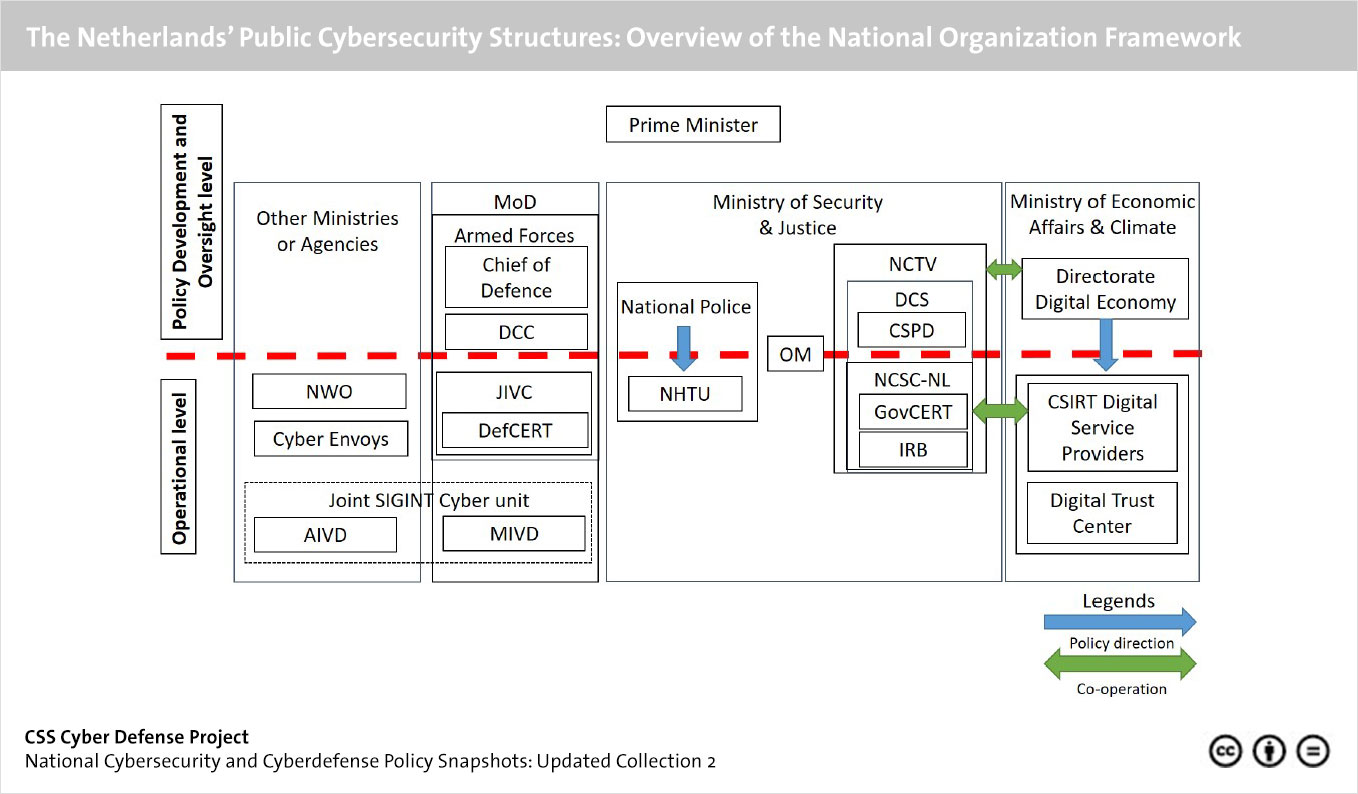
\includegraphics[width=1\textwidth]{Images/netherlands.jpg}
    \caption{\textit{Netherlands Cyber Structure}}
        \source{Source: \autocite{sdewar_2018_national}}
    \label{fig:netherlands}
\end{figure}

\textbf{Public-Private collaboration} Due to the interconnection between digital services and infrastructure in both the public and private spheres, the Netherlands has established the Nationwide Network of Cybersecurity Partnership (LDS), which will be further developed in the future. The aim of this entity is to facilitate and improve the sharing of information \autocite{ministryofjusticeandsecurity_2022_netherlands}. Another important step toward a more secure infrastructure and cyber environment involves the need to apply the secure-by-design principle to both hardware and software assets. EU regulations, such as the Cyber Resilience Act and Cybersecurity Act, will impose strict rules to guarantee the security of ICT products throughout their lifecycle. Furthermore, the Netherlands has prepared a National Plan for Digital Incidents to effectively respond to potential cyber threats and crises in the digital domain. This comprehensive plan outlines the necessary strategies and actions to be taken in the event of a digital incident, ensuring a coordinated and swift response. 

\textbf{Intelligence gathering} The Netherlands has developed intelligence gathering capabilities. Important information is regularly exchanged with its partners, aligned with the proposed objectives. Additionally, the Defence Intelligence and Security Service (DISS) plays a crucial role in providing intelligence on cyber threats to various entities, including Defence, DefCERT, the Public Prosecution Service, the National Cyber Security Centre (NCSC), and the private sector. The DISS contributes to the National Detection Network (NDN) to detect and respond to cyber espionage and sabotage, collaborating with other organizations. The DISS's intelligence forms the basis for offensive cyber capabilities and allows for proactive defence measures. Furthermore, increasing intelligence capabilities will enable the Netherlands to assess the attribution of the attack more precisely, making the country less attractive for attacks \autocite{theinternationalinstituteforstrategicstudies_2023_cyber, ministryofdefence_2018_defence}.

\textbf{Offensive \& Defensive capabilities} In the context of Cyberstrategy 2022-2028, it is claimed that the government possesses both offensive and defensive cyber capabilities, demonstrating effectiveness in both peacetime and wartime scenarios \autocite[38]{ministryofjusticeandsecurity_2022_netherlands}. While the specific details of these capabilities remain undisclosed for security reasons, the document provides insight into the overarching doctrine and strategies that could be employed. Notably, the document acknowledges the potential utilisation of criminal and non-criminal assets to counteract and disrupt cyberattackers, presenting a diplomatic stance on the Netherlands' possession and potential deployment of offensive (destructive) cyber capabilities. The Netherlands has been developing offensive cyber capabilities, reflecting a proactive approach to countering cyber threats. The International Institute of Strategic Studies highlights joint efforts by DCC and MIVD to develop these capabilities, including involvement in \textit{ defend forward} strategies, where foreign malware is actively addressed to prevent potential attacks on national security \autocite{theinternationalinstituteforstrategicstudies_2023_cyber}. However, the National law framework does not allow the application of those capabilities in peacetime. 

A significant development related to this stance occurred on December 2, 2022, when the cabinet introduced a bill titled \textit{Temporary law on AIVD and MIVD investigations into countries with an offensive cyber programme} to the House of Representatives. This legislative initiative is a direct response to operational challenges faced by the General Intelligence and Security Service (AIVD) and the Military Intelligence and Security Service (MIVD) in conducting investigations into cyber threats originating from state actors \autocite{nationalgovernmentofthenetherlands_2023_internationale}. This legislative proposal signifies the government's commitment to addressing operational bottlenecks and underscores the evolving nature of its cyber defence and offence strategies in the face of emerging threats.

From an organisational perspective, the Netherlands is promoting the establishment of Joint Cyber Mission Teams. Their role will expedite the integration of cyber weapons in a wartime scenario. The teams will be made up of personnel with diverse experience, bringing together individuals from DISS and the armed forces. This collaborative approach recognises the complementary nature of the knowledge and skills required for effective intelligence and military operations in the cyber domain. To enhance transparency and awareness of cyber operationalisation in military missions, Article 100 of the Constitution will be updated with additional statements regarding the cyber domain. The deterrence strategy is not only based on the denial effect through proactive defence, but also with the possibility of using cyber military means to respond to the attacker (known as deterrence by punishment). 

\textbf{Education & Investments} The government's strategic priorities to enhance cybersecurity awareness, education, and expertise are integral to the Cybersecurity Strategy for the 2022-2028 period. Recognising the shared responsibility for digital product security, the government aims to increase awareness among the public and SMEs through targeted information campaigns. To foster a cyber-resilient future, the curriculum for primary and secondary education will include core objectives on cybersecurity skills. The collaboration extends to the labour market, where the government is working with educational institutions and the business community to implement upskilling and reskilling programs. Investments in higher professional education, specifically in the sciences and cybersecurity, focus on increasing admission, reducing dropout rates, facilitating lateral entry, and ensuring a smooth transition to the labour market. This comprehensive approach reflects the government's commitment to building a digitally literate and secure society. Furthermore, the government invested €111 million in cyber resilience, involving the strengthening of critical infrastructure, intelligence agencies, and the improvement of both defence cyber capabilities and an increase in the number of cyber diplomats \autocite{nationalgovernmentofthenetherlands_2023_internationale}. Like other countries analysed, the cybersecurity labour market remains a critical requirement to implement a coherent and efficient cyberstrategy.

\textbf{Cyber-Kinetic Integration} The Netherlands is contributing to the development and implementation of the integration of cyber weapons in NATO missions \autocite{ministryofdefence_2018_defence} Firstly, the country is integrating its IT systems within the Defence organization, encompassing management, command, sensor, and weapon systems. The integration has dual outcomes: on one side, it increases the attack vectors and makes the infrastructure more vulnerable. Yet, on the other hand, it provides a strategic advantage by creating a unified and synchronized approach to military operations. The establishment of a cyber defence command \autocite{theinternationalinstituteforstrategicstudies_2023_cyber} highlights the importance that the Netherlands places on cybersecurity in military affairs.  

\textbf{Cyber Diplomacy} The Netherlands has been a pioneer in applying diplomatic responses to cyberattacks. In accordance with the EU Cyber Diplomacy Toolbox, the country not only responds with sanctions and public declarations against state actors behind cyberattacks, but also counters influence operations actively using cyberattacks and social engineering to shape public opinion, a situation known as hybrid wars. For this reason, the Netherlands strongly believes in the creation of international and European political alliances to counter these threats. In fact, European tools such as the Hybrid Toolbox and the Foreign Information Manipulation and Interference Toolbox, despite their independent nature, can strengthen connections, making it possible to act more effectively and combat fragmentation \autocite{nationalgovernmentofthenetherlands_2023_internationale}.

\newpage

\section{Discussion}
France, Estonia, Germany, and the Netherlands are well qualified and equipped countries to counter cyberattacks, even in emergencies and crises such as war. As advanced and technology-driven economies, the expectation was not to find a lower level than the cases observed in Ukraine, but rather to determine if and how their strategies encompass the risks that we have identified as lessons to be learnt from the war in Ukraine.

The results were twofold. When analysing public documents, it is evident that these countries are structurally prepared and pay specific attention to their IT and critical infrastructure. They also emphasize the role of deterrence and political alliances through the European Union, NATO, and international fora. However, limited information was available regarding the integration of cyber capabilities into military missions.

\begin{figure}[H]
    \centering
    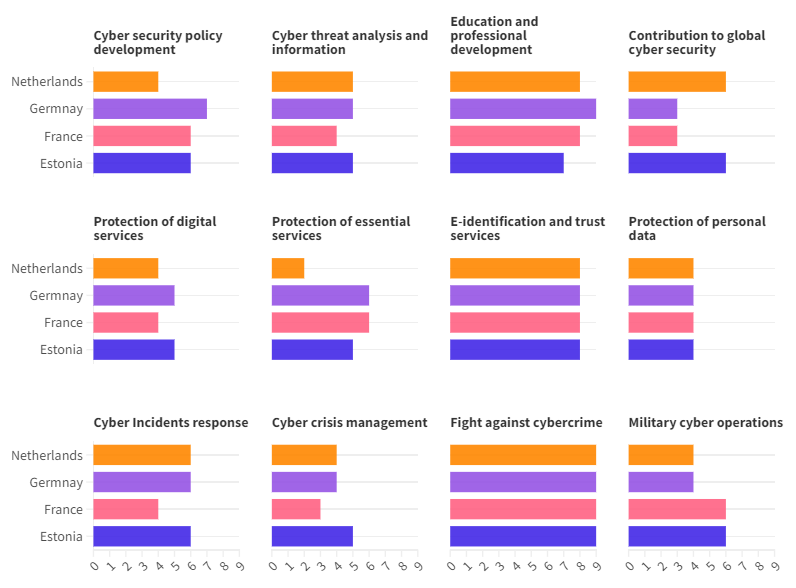
\includegraphics[width=1\textwidth]{Images/ncsi_index.png}
    \caption{\textit{National Cyber Security Index Comparison}}
        \source{Source: \autocite{egovernmentacademy_2023_ncsi}, Author's representation}
    \label{fig:ncsi_index}
\end{figure}

\newpage
\textbf{The National Cyber Security Index}
The Figure \ref{fig:ncsi_index} confirms the analysis performed. Estonia emerges as the leading country in overall cybersecurity, scoring 93.51 out of 100. This is attributed to its robust cybersecurity policy development, high-level cyber threat analysis, and information sharing capabilities. Germany follows closely with a score of 90.91, showcasing strengths in education, professional development, and global contributions to cybersecurity. France, with a score of 84.42, demonstrates a solid foundation in cybersecurity policy and global contribution but lags in some areas like cyber crisis management. The Netherlands, scoring 83.12, excels in education and professional development but faces challenges in the protection of essential services and e-identification. However, the methodology used for computing National Cyber Security Index have issues that have been addressed for the post September 2023 analysis. Similar results have been found with the National Cyber Power Index, confirming the role of intelligence gathering capabilities of the country analysed as the main cyber capability. 

\textbf{Political Alliances and the role of European Union}

All four countries recognise the role of the European Union as a catalyst to enhance cooperation in the cyber domain. The regulatory power of the European Union is shaping how national strategies are implemented. For instance, NIS2 will oblige more than 5,000 private companies in the Netherlands to report cyber incidents and comply with EU regulations. This expansion of players directly affects the amount of information that will be processed, underscoring the importance of entities that facilitate information sharing and cooperation among various actors.

Furthermore, the prominent role of NATO in the cyber domain constitutes a real deterrent for these countries and influences the implementation of cyber capabilities in the military field. Even with the European Union's engagement in the military field through its PESCO missions, specifically addressing the cyber domain (such as the Cyber Range and the Enhancement of C2 structures), the analysed strategies of the countries indicate that the EU is predominantly viewed as a catalyst concerning civilian aspects, critical infrastructure certification, and broader cross-country risk management.

\textbf{Offensive-Defensive Cyber Capabilities}

Continuing from the previous discussion, the distinction between offensive and defensive cyber capabilities often arises from political considerations, reflecting the broader national security strategies of individual countries. While the underlying skills required for offensive and defensive operations are often similar, the decision to formally establish military doctrines for cyberspace varies among nations. In the cases of the Netherlands and Estonia, the absence of a defined military doctrine may suggest a pragmatic approach, potentially driven by their relatively smaller size, agility, and the rapidly evolving nature of cyber threats. This approach allows these countries the flexibility to adapt quickly to emerging challenges and leverage international collaborations. Conversely, France and Germany's decision to define and implement military doctrines demonstrates a commitment to a structured and proactive stance in cyberspace. These doctrines provide a clear framework for coordinated responses, delineating roles and responsibilities to enhance national cybersecurity.

Across the countries discussed, it is evident that all possess capabilities in both offensive and defensive cyber operations, although the extent to which these capabilities are emphasized and utilized varies. Germany stands out for its political stance, actively refraining from employing its offensive cyber capabilities. This strategic decision aligns with a cautious approach, possibly influenced by political considerations and the prevailing legal framework. In contrast, Estonia is actively advancing its offensive capabilities as a deterrent, showcasing a proactive strategy to dissuade potential adversaries. The Netherlands is in the process of fortifying its national legal framework to facilitate norm-setting for cyber operations, underscoring its commitment to responsible and regulated cyber activities. France adopts a more balanced approach, with defined military doctrines for both offensive and defensive cyber operations. Despite the absence of concrete evidence of offensive cyber actions in the real world, these countries collectively prioritize defensive capabilities. This emphasis can be attributed to political considerations, the absence of active warfare, and a shared recognition of the importance of protecting national interests in the evolving digital landscape.

On the other hand, it is undeniable that these countries are actively preparing for the potential deployment of such capabilities. Moreover, NATO military exercises, including Crossed Swords and others conducted in the Baltic region, along with the PESCO mission, with a specific emphasis on Command \& Control missions, serve as clear indicators that NATO and EU member states are engaging in training, exploration, and the implementation of cyber-kinetic integration. The specifics of this domain warrant further exploration, particularly as more publicly available information becomes accessible. Among these nations, the Netherlands stands out as it has made some references to cyber-kinetic integration in its national documentation, while referring to the integration of IT infrastructure with other military assets (sensors, radars, among others).

\textbf{Role of War in Ukraine}

Even though the war in Ukraine has led to increased funding for the defense sector in Europe, this has not directly translated into enhanced resources for the cyber domain. Germany and the Netherlands, with their newly published cyber strategies following the outbreak of the war, have earmarked additional funds to bolster their preparedness and infrastructure. From a political standpoint, there appears to be a divergence in how the Ukraine War has influenced the shaping of defense strategies. France has assumed a more cautious stance, focusing its policy on the long term without specific cases mentioned. In contrast, Estonia and the Netherlands emphasize the war's role. Particularly, Estonia has formulated a strategy to ensure the functioning of its e-Government and critical information infrastructure even if it loses control of its territory (a more diplomatic way of stating in the event of a Russian invasion). Meanwhile, the Netherlands has increased its budget allocation to enhance cyber capabilities and assist international partners in countering state-sponsored operations.

\textbf{Challenges}

The predominant challenge shared by all the countries is their ability (or lack thereof) to attract the necessary skills crucial for both cyber defence and offensive operations. Various factors contribute to this issue. Many skilled professionals prefer opportunities in the private sector, where salaries and benefits may be more lucrative. However, a noteworthy shift is occurring, with a recent trend toward adopting a less traditional military or law enforcement approach to cyber defence. Estonia serves as a noteworthy example with its Cyber Defence Unit, demonstrating the acceptance of civilians who can contribute significantly to cybersecurity efforts.

Another contributing factor to the skills gap is evident in the education sector. Only in recent years have university courses dedicated to cybersecurity and a multidisciplinary approach to cyberspace securitization emerged. Notably, the Netherlands and Estonia have taken a leading role in Europe in cultivating educational programs in this field. However, addressing this challenge necessitates further investment and commitment to expanding educational initiatives, fostering collaboration between academia and industry, and promoting the development of a skilled workforce equipped to navigate the complex landscape of cybersecurity.

Another challenge that has emerged is the cooperation between the public and private sectors. All the countries have developed frameworks and entities to facilitate information sharing and the implementation of best practices. While this strategy may work with large companies, it struggles to be applied to SMEs. This is why Estonia and the Netherlands have created projects to promote a cyber culture within civil society and the private sector.

In summary, the evolving landscape of cybersecurity in these European nations is influenced by a dynamic interplay of geopolitical, technological, and strategic factors. Ongoing efforts to navigate these challenges will shape their resilience and effectiveness in the face of emerging cyber threats.

